\documentclass[12pt, letterpaper]{article}
\usepackage[titletoc,title]{appendix}
\usepackage{color}
\usepackage{booktabs}
\usepackage[usenames,dvipsnames,svgnames,table]{xcolor}
\definecolor{dark-red}{rgb}{0.75,0.10,0.10}
\definecolor{bluish}{rgb}{0.05,0.05,0.85}
\PassOptionsToPackage{unicode}{hyperref}
\PassOptionsToPackage{naturalnames}{hyperref}
\usepackage[margin=1in]{geometry}
\usepackage[linkcolor=blue,
            colorlinks=true,
            urlcolor=blue,
            pdfstartview={XYZ null null 1.00},
            pdfpagemode=UseNone,
            citecolor={bluish},
            pdftitle={social proof}]{hyperref}

%\newcites{SI}{SI References}
\usepackage{natbib}

\usepackage{float}
\usepackage{placeins}

\usepackage{geometry}  % see geometry.pdf on how to lay out the page. There's lots.
\geometry{letterpaper} % This is 8.5x11 paper. Options are a4paper or a5paper or other...
\usepackage{graphicx}  % Handles inclusion of major graphics formats and allows use of
\usepackage{amsfonts,amssymb,amsbsy}
\usepackage{amsxtra}
\usepackage{verbatim}
%\setcitestyle{round,semicolon,aysep={},yysep={;}}
\usepackage{setspace} % Permits line spacing control. Options are:
%\doublespacing
%\onehalfspace
%\usepackage{sectsty}    % Permits control of section header styles
\usepackage{pdflscape}
\usepackage{fancyhdr}   % Permits header customization. See header section below.
\usepackage{url}        % Correctly formats URLs with the \url{} tag
\usepackage{fullpage}   %1-inch margins
\usepackage{multirow}
\usepackage{verbatim}
\usepackage{rotating}
\setlength{\parindent}{3em}

%\usepackage[T1]{fontenc}
%\usepackage[bitstream-charter]{mathdesign}

\usepackage{chngcntr}
\usepackage{longtable}
\usepackage{adjustbox}
\usepackage{dcolumn}

\usepackage[nameinlink, capitalize, noabbrev]{cleveref}

\def\citeapos#1{\citeauthor{#1}'s (\citeyear{#1})}

\makeatother

\usepackage{footmisc}
\setlength{\footnotesep}{\baselineskip}
\makeatother
\renewcommand{\footnotelayout}{\normalsize \doublespacing}


% Colors
\usepackage{color}

\newcommand{\bch}{\color{blue}\em  }   % begin change
\newcommand{\ying} {\color{orange}\em  }   % begin change
\newcommand{\bgcd} {\color{purple}\em }
\newcommand{\ech}{\color{black}\rm  }    % end change

% Caption
\usepackage[hang, font=small,skip=0pt, labelfont={bf}]{caption}
%\captionsetup[subtable]{font=small,skip=0pt}
\usepackage{subcaption}

% tt font issues
% \renewcommand*{\ttdefault}{qcr}
\renewcommand{\ttdefault}{pcr}


\usepackage{tocloft}


\usepackage{lscape}
\renewcommand{\textfraction}{0}
\renewcommand{\topfraction}{0.95}
\renewcommand{\bottomfraction}{0.95}
\renewcommand{\floatpagefraction}{0.40}
\setcounter{totalnumber}{5}
\makeatletter
\providecommand\phantomcaption{\caption@refstepcounter\@captype}
\makeatother

\title{Is an Uncertain Prospect Less Preferred Than Its Worst Possible Outcome? New Evidence on the Uncertainty Effect\thanks{You can download the replication materials from \href{http://github.com/soodoku/uncertainty}{http://github.com/soodoku/uncertainty}.}}


\author{Doug Ahler\thanks{Doug can be reached at, \href{mailto:doug.ahler@gmail.com}{\footnotesize{\texttt{doug.ahler@gmail.com}}}} \and Gaurav Sood\thanks{Gaurav can be reached at \href{mailto:gsood07@gmail.com}{\footnotesize{\texttt{gsood07@gmail.com}}}}}

\date{\today}

\begin{document}
\maketitle

\thispagestyle{empty}
\begin{abstract}
\noindent In a seminal article in the \textit{Quarterly Journal of Economics}, \cite{gneezy2006uncertainty} (GLW) report the discovery of the uncertainty effect. In a series of experiments, the authors find that people are averse to picking the uncertain option even when the certain choice is worse than the worst possible outcome of the uncertain option. We successfully replicate the main finding with two larger, more representative surveys. But our data suggest three qualifiers: 1. adding a phrase that clarifies that people are guaranteed to get at least the worst option or asking people to estimate the expected value of the uncertain option before choosing reduces the effect, 2. rephrasing the uncertain option in terms of natural frequencies undoes the effect, and 3. redoing the experiment with monetary choices also undoes the effect.
\end{abstract} 
\clearpage
\setcounter{page}{1}
\doublespace

\section*{Experiment 1}

We conducted our first survey on Lucid \citep{coppock2019validating}. We recruited 800 participants of whom 674 passed the attention check. (See the SI for details.) Our analyses are limited to those who passed the attention check.

Our experiment has four treatment arms. The first two replicate the treatment arms in one of the experiments in GLW. In the first condition, we asked respondents if they would prefer \$25 in cash or a \$50 Amazon gift card. We call it the \textbf{Certain Choice} condition. We compare this to a second \textbf{Uncertain Choice} condition in which respondents were asked whether they would prefer \$25 in cash or a lottery in which they had a 50\% chance of winning a \$50 Amazon gift card and a 50\% chance of winning a \$100 Amazon gift card. Since the expected value of this lottery is \$75 in Amazon money, the rational expectation is that more participants will take the Amazon gift card in this condition. However, \cite{gneezy2006uncertainty} find that people take cash at a higher rate in the lottery condition, apparently because they are averse to uncertainty.

Our next two conditions probe alternate mechanisms for the effect. It is possible that the wording about the lottery is confusing. Perhaps some participants believe the lottery is sequential, i.e., they first have a chance of winning \$50 and then a chance of winning \$100 and, thus, a chance of winning nothing at all. To preclude this reasoning, we introduced a third condition in which participants chose between \$25 in cash or the lottery in the second condition, but with a clarification attached to the lottery: ``To be clear, you are guaranteed to get at least a \$50 gift card.'' If participants are truly averse to uncertainty, we should see similar (and relatively small, compared to the baseline) proportions opting for the lottery in both the \textbf{Uncertain Choice} and \textbf{Clarifying Uncertain Choice} conditions. But if confusion about the lottery explains any of the irrational choices in the \textbf{Uncertain Choice} condition, we should see higher proportions opting for the lottery in the \textbf{Clarifying Uncertain Choice} condition.

Lastly, based on the idea (spoken about by GLW) that comparison across different units (gift card vs. cash) may be an essential condition for the effect to hold, we offered a \textbf{Direct Comparison} condition that asked respondents to choose between a \$50 Amazon gift card and the regular lottery. Unlike other arms that offer a lottery, this experimental arm has a certain choice that is more commensurate with the second option in \textbf{Certain Choice} than the first. It also makes inference difficult. It could be that fewer respondents choose the lottery because the trade-off is harder or it could be that more respondents choose the lottery because the comparison is clearer. Because of these inferential issues, we exclude this condition.

Figure \ref{fig:exp_1_lucid} presents the results. In the \textbf{Certain Choice} condition, just 36.5\% of the participants opt for the \$25 in cash over the \$50 Amazon gift card. Since the lottery is worth more than \$50 in Amazon gift card, we should expect a smaller percentage to take the cash. But we observe a different pattern. First, a full 61.5\% opt for cash over the lottery in the original \textbf{Uncertain Choice} condition. Consistent with \citet{gneezy2006uncertainty}, we find that the lottery worth \$75 in Amazon gift card, and guaranteed to pay out at least a \$50 Amazon gift card, is less popular than \$50 in Amazon gift card in the \textbf{Certain Choice}.

\begin{figure}[h]
    \centering
    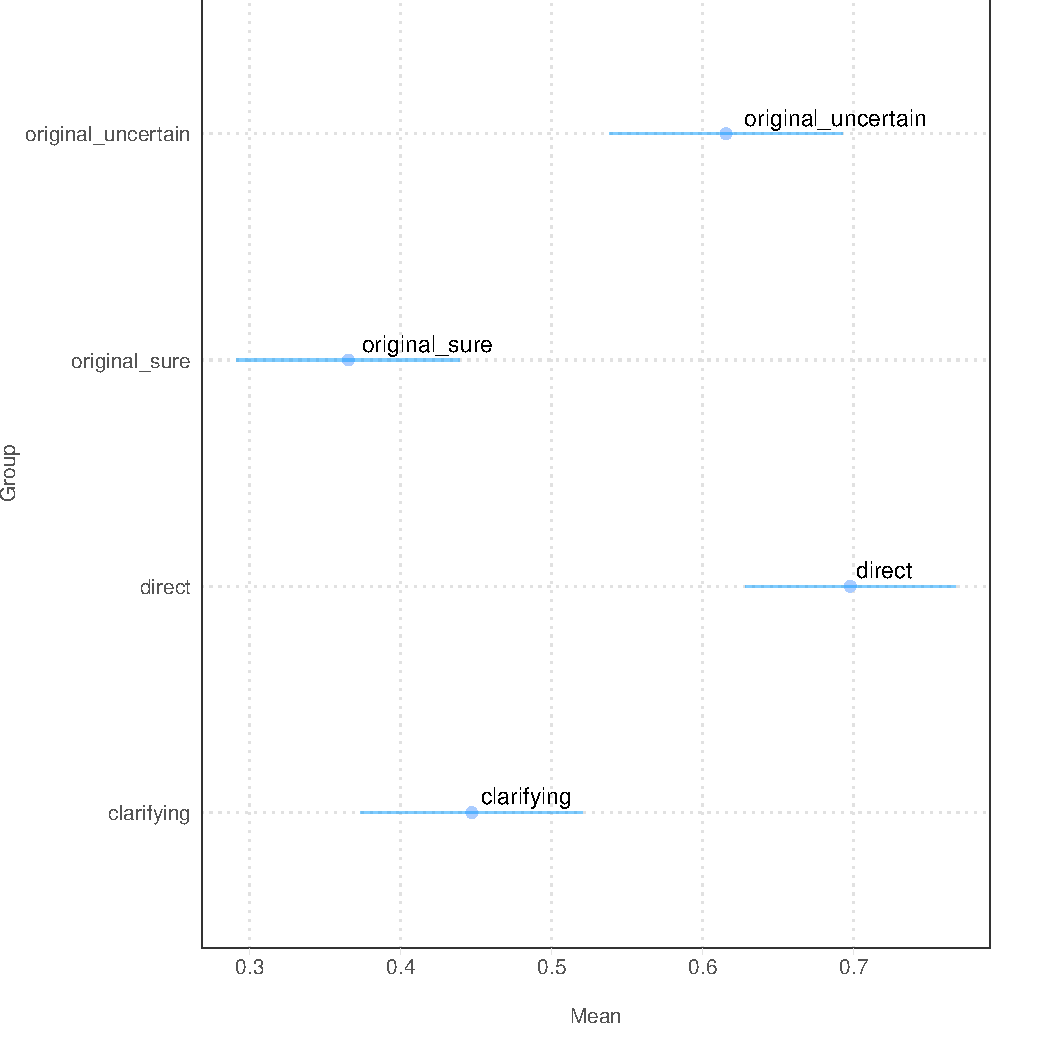
\includegraphics{figs/lucid_exp.pdf}
    \caption{Experiment 1 (Lucid)}
    \label{fig:exp_1_lucid}
\end{figure}

As noted above, this could be due to confusion over how the lottery is described. Adding the ``clarification'' causes a dramatic drop in people choosing \$25 in cash. In the \textbf{Clarifying} condition, 44.7\% take the \$25 in cash. Thus, unclear wording surrounding the lottery may explain a significant portion of the uncertainty effect.

\section*{Experiment 2 (Prolific)}

We conducted our second study on Prolific \citep{palan2018prolific}. We recruited 853 participants, of which 814 passed the attention check. We limit our analyses to those who passed the attention check. (See the SI for details.)

The first experiment had four treatment arms starting with the \textbf{Certain Choice} and \textbf{Uncertain Choice} conditions similar to the ones in GLW. Our third condition examined whether it was the clarity with which we stated the uncertain option that caused respondents to avoid it. So we phrased it in terms of natural frequencies \citep{gigerenzer2011natural}. We call the condition \textbf{Natural Frequencies}. Lastly, we created a treatment arm in which we offered a decoy choice to structure the preferences underlying the choice \citep{ariely2008predictably}. We label the condition \textbf{Decoy Choice}.

For the second experiment, we used the ruse of offering choices for how the bonus should be delivered. (There was a slew of questions about another topic separating the two experiments.) Once again we had two conventional arms --- \textbf{Certain} and \textbf{Uncertain}. In the third condition, we asked respondents to estimate the expected value of the uncertain option before making the choice. We constructed this choice to direct respondents' gaze toward a particular number that we felt would help respondents overcome their System 1 thinking.

Figure \ref{fig:exp_1_prolific} presents the results of the first experiment. Once again, we see a large difference in people choosing \$25 in cash between the \textbf{Certain} and the \textbf{Uncertain} condition, as predicted by GLW. Offering a decoy choice doesn't affect the propensity to choose the \$25 in cash in a way we can detect confidently. However, the natural frequencies formulation leads to a dramatic reduction in people choosing \$25 in cash, with it coming at roughly the same level as in the \textbf{Certain} option.

\begin{figure}[h]
    \centering
    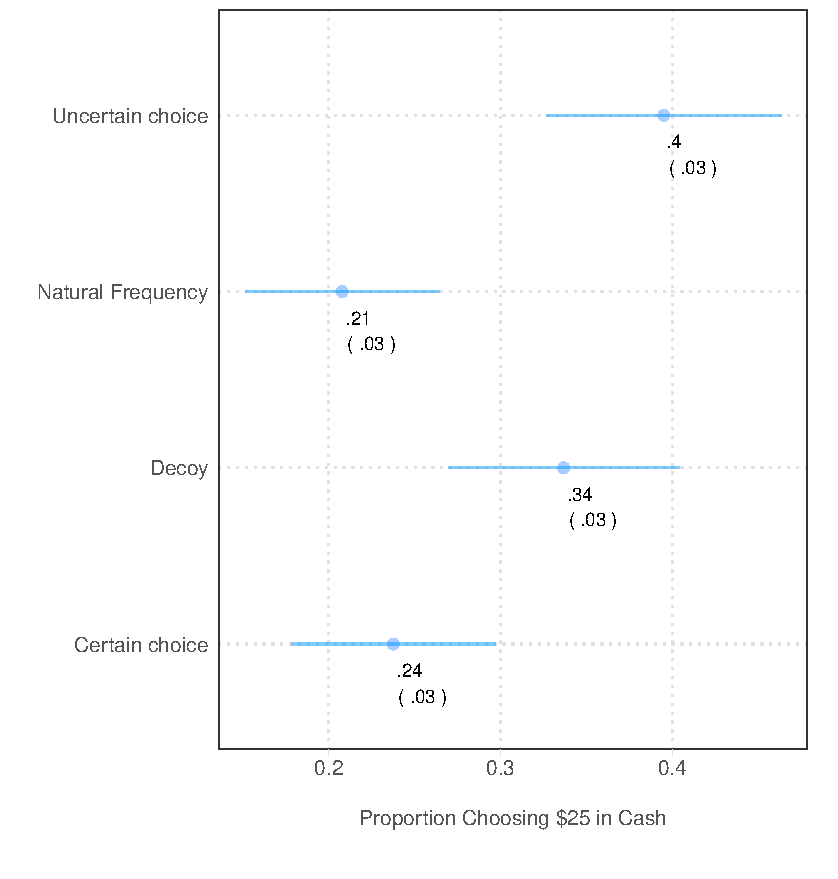
\includegraphics{figs/prolific_exp1.pdf}
    \caption{Experiment 1 (Prolific)}
    \label{fig:exp_1_prolific}
\end{figure}

The results of the second experiment suggest there is no uncertainty effect when people are incentivized. In the \textbf{Certain choice} condition, 64\% of the respondents chose the \$.25 in cash option. This percentage \textit{declines} in the \textbf{Uncertain choice} condition with just about 48\% of the respondents choosing the option. The \textbf{Ask} condition results sit somewhere between the \textbf{Certain choice} and \textbf{Uncertain choice} with about 54\% of the respondents choosing the \$.25 in cash.

\begin{figure}[h]
    \centering
    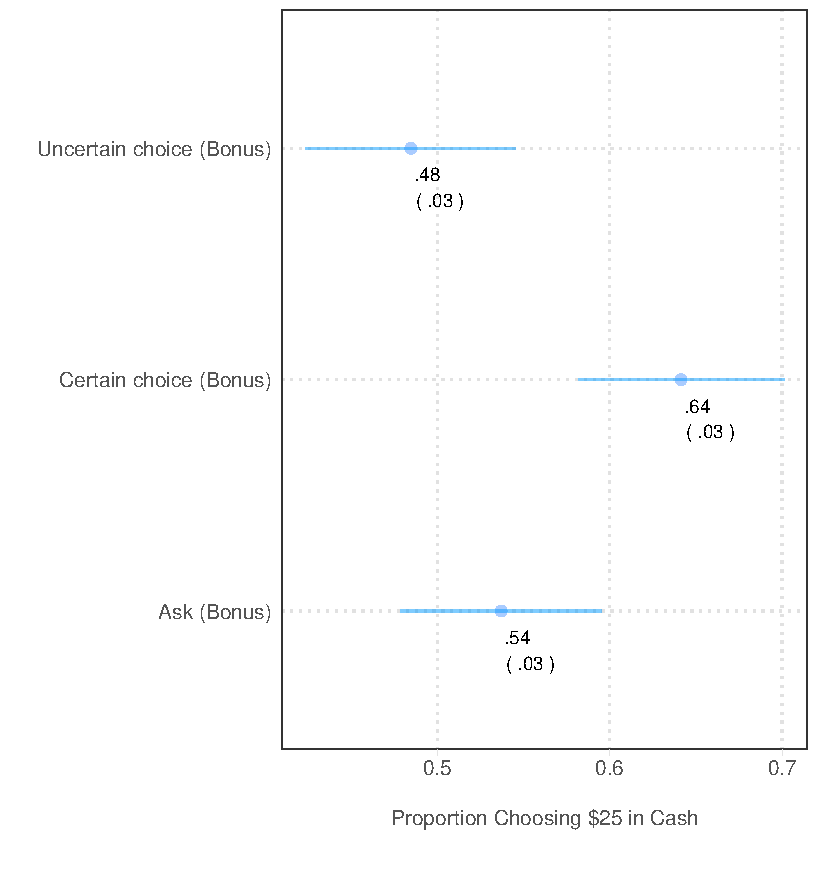
\includegraphics{figs/prolific_exp2.pdf}
    \caption{Experiment 2 (Bonus) (Prolific)}
    \label{fig:exp_2_prolific}
\end{figure}
\clearpage
\bibliographystyle{apsr}
\bibliography{uncertainty}
\clearpage

%===============================================================================
%===============================================================================
% Appendix
%===============================================================================
%===============================================================================
\appendix
\renewcommand{\thesection}{SI \arabic{section}}
\renewcommand\thetable{\thesection.\arabic{table}}  
\renewcommand\thefigure{\thesection.\arabic{figure}}
\counterwithin{figure}{section}
\counterwithin{table}{section}

\section*{Supporting Information}\label{si}

\section{Survey 1 (Lucid)}

\subsection{Attention Check}
People are very busy these days and many do not have time to follow what goes on in the government. We are \textbf{\underline{testing whether people read questions.}} To show that you've read this much, answer \textbf{\underline{both}} ``extremely interested'' and ``very interested.'' --- Extremely interested, Very interested, Moderately interested,  Slightly interested, Not at all interested

\subsection{Numeracy Battery}

The order of the response options was randomized.

\begin{itemize}
    \item A man writes a check for $100 when he has only $70.50 in the bank. By how much is he overdrawn? — \$29.50, \$170.50, \$100, \$30.50
    \item Imagine that we roll a fair, six-sided die 1000 times. Out of 1000 rolls, how many times do you think the die would come up as an even number? — 500, 600, 167, 750
    \item If the chance of getting a disease is 10 percent, how many people out of 1,000 would be expected to get the disease? — 100, 10, 1000, 500
    \item In a sale, a shop is selling all items at half price. Before the sale, the sofa costs \$300. How much will it cost on sale? — \$150, \$100, \$200, \$250
    \item A second-hand car dealer is selling a car for \$6,000. This is two-thirds of what it cost new. How much did the car cost new? — \$9,000, \$4,000, \$12,000, \$8,000
    \item In the BIG BUCKS LOTTERY, the chances of winning a \$10 prize are 1\%. What is your best guess about how many people would win a \$10 prize if 1000 people each buy a single ticket from BIG BUCKS? — 10, 1, 100, 50
\end{itemize}

\subsection{Experimental Conditions}

\begin{itemize}
    \item \textbf{Certain Choice.} Which would you prefer? \$25 in cash, A \$50 Amazon gift card
    
    \item \textbf{Uncertain Choice.} Which would you prefer? \$25 in cash, A lottery in which you have a 50\% chance of winning a \$50 Amazon gift card and a 50\% chance of winning a \$100 Amazon gift card.
    
    \item \textbf{Uncertain Worst Case Choice.} Which would you prefer? \$25 in cash, A lottery in which you have a 50\% chance of winning a \$50 Amazon gift card and a 50\% chance of winning a \$100 Amazon gift card. To be clear, you are guaranteed to get at least a \$50 gift card.

    \item \textbf{Direct Comparison.} Which would you prefer? \$A \$50 Amazon gift card, A lottery in which you have a 50\% chance of winning a \$50 Amazon gift card and a 50\% chance of winning a \$100 Amazon gift card.
    
\end{itemize}

After the \textbf{Uncertain Choice} and the \textbf{Uncertain Worst Case Choice} condition, we asked a follow-up question:  What is the average amount (in gift card money) you would win from the following lottery? You have a 50\% chance of winning a \$50 gift card and a 50\% chance of winning a \$100 gift card.

\section{Survey 2 (Prolific)}

\subsection{Attention}

\subsubsection{Incentivizing Attention}
On the survey, we will check if people are paying attention. Those paying attention will get an additional bonus payment.

\subsubsection{Attention Check}
People are very busy these days and many do not have time to follow what goes on in the government. We are \textbf{\underline{testing whether people read questions.}} To show that you've read this much, answer \textbf{\underline{both}} ``extremely interested'' and ``very interested.'' --- Extremely interested, Very interested,  Moderately interested, Slightly interested, Not at all interested

\subsection{Numeracy Battery}

The order of the response options was randomized.

\begin{itemize}
    \item In the BIG BUCKS LOTTERY, the chances of winning a \$10 prize are 1\%. What is your best guess about how many people would win a \$10 prize if 1000 people each buy a single ticket from BIG BUCKS? — 10, 1, 100, 50
    
    \item A train travels 1 mile in 1 minute and 20 seconds. How many miles will it travel in one hour? — 45, 60, 40, 50
    
    \item Imagine that we roll a fair, six-sided die 1000 times. Out of 1000 rolls, how many times do you think the die would come up as an even number? — 500, 600, 167, 750
    
    \item In a sale, a shop is selling all items at half price. Before the sale, the sofa costs \$300. How much will it cost on sale? — \$150, \$100, \$200, \$250
    
    \item A second-hand car dealer is selling a car for \$6,000. This is two-thirds of what it cost new. How much did the car cost new? — \$9,000, \$4,000, \$12,000, \$8,000
    
    \item A father is 33 years older than his son. The father is also four times as old as his son. What's the father’s age? — 44, 33, 53, 62
\end{itemize}

\subsection{Experimental Conditions}

\begin{itemize}
    \item \textbf{Gigerenzer Choice.} Which one do you prefer? \$25 in cash, An Amazon gift card whose value is decided by the following lottery: Of every 100 people who play the lottery, 50 win a \$50 Amazon gift card and the other 50 win a \$100 Amazon gift card.
    
    \item \textbf{Ariely Choice.} Which one do you prefer? A lottery in which you have a 60\% chance of winning a \$50 Amazon gift card and a 40\% chance of winning a \$100 Amazon gift card., \$25 in cash,  A lottery in which you have a 50\% chance of winning a \$50 Amazon gift card and a 50\% chance of winning a \$100 Amazon gift card.

    \item \textbf{Certain Choice.} Which one do you prefer? \$25 in cash, \$50 Amazon gift card
    
    \item \textbf{Uncertain Choice.} Which one do you prefer? \$25 in cash, A lottery in which you have a 50\% chance of winning a \$50 Amazon gift card and a 50\% chance of winning a \$100 Amazon gift card.
\end{itemize}

Experiment 2 (Bonus)

\begin{itemize}
    \item \textbf{Certain Choice with Bonus.} You are eligible for the bonus payment. You can pick one of the following options for your bonus ... \$0.25 in cash,  An Amazon gift card of \$0.50 in value

    \item \textbf{Uncertain Choice.} You are eligible for the bonus payment. You can pick one of the following options for your bonus ... \$0.25 in cash, An Amazon gift card whose value is determined by a virtual coin toss. You win a \$0.50 Amazon gift card if the coin lands heads and a \$1 Amazon gift card if it lands tails

    \item \textbf{Ask and Choose with Bonus.} What is the lowest amount of money that you would get from a lottery where you have a 50\% chance of winning \$50 and a 50\% chance of winning \$100? You are eligible for the bonus payment. You can pick one of the following options for your bonus .. \$0.25 in cash,  An Amazon gift card whose value we determine by a lottery where a person has a 50\% chance of winning a \$0.50 Amazon gift card and a 50\% chance of winning a \$1 Amazon gift card
\end{itemize}

\section{Figures}

\begin{figure}[h]
    \centering
    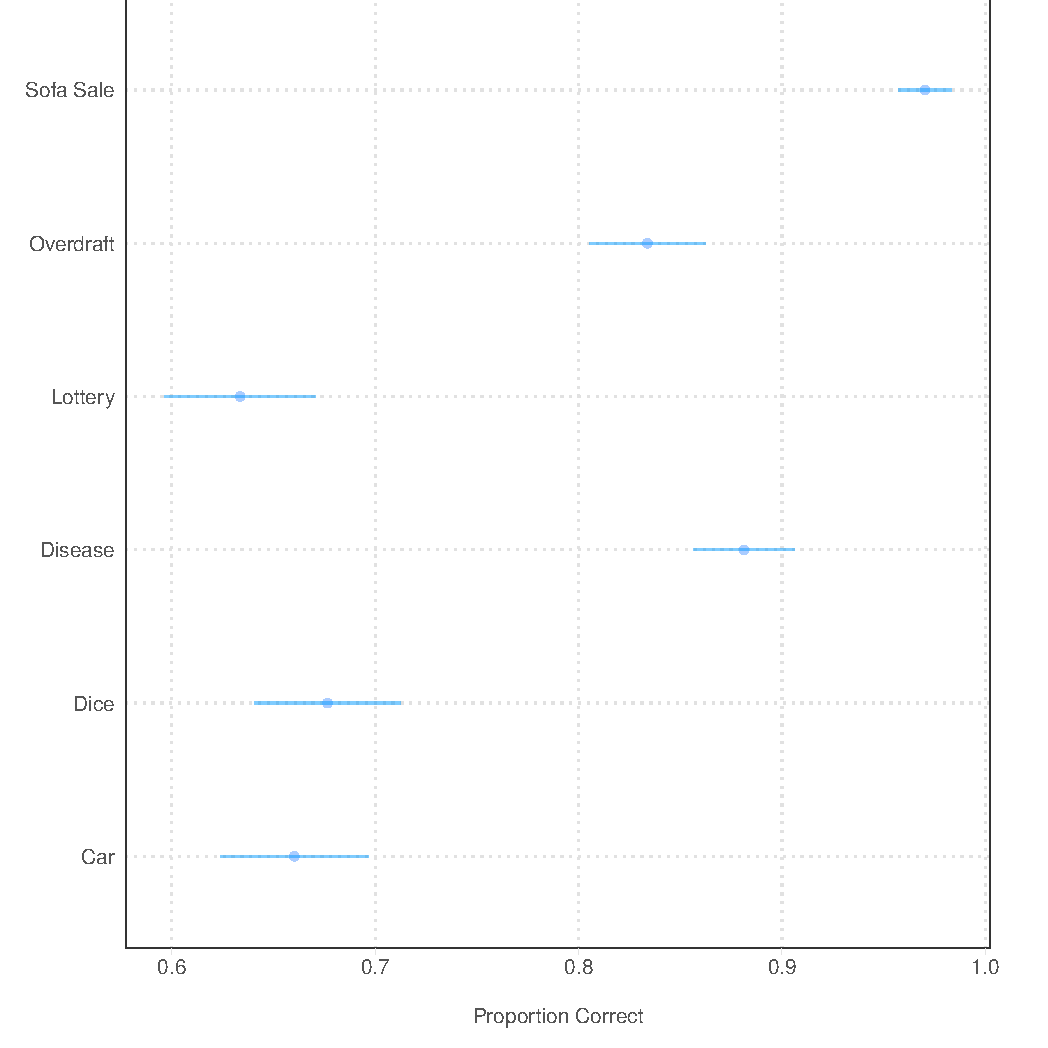
\includegraphics{figs/lucid_numeracy.pdf}
    \caption{Numeracy}
    \label{fig:lucid_numeracy}
\end{figure}
\end{document}
